\subsection{Tilt Wing}
\label{tiltwing}
%Description about it
A tilt-wing (or tilt-tail/canard) mechanism is a common feature of numerous conceptual designs, including the two conceptual designs being pursued for further analysis. The following analysis assumes a concept with a single tilt wing with individually actuated port and starboard wings. If necessary, a similar approach/design could be utilised for a simpler tilt wing mechanism which rotates both port and starboard wings in unison. 

\subsubsection{Theory}
%What is required by the system
Tilt-wing UAVs incorporate a novel system that presents various beneficial design properties and performance merits. Research focus on developing aircraft with long-distance efficiency and VTOL capabilities has highlighted the effective use of tilt-rotors and tilt-wings by allowing motors to be used in both flight configurations, improving power efficiency and reducing unnecessary weight. Rotating the wing in parallel with the motor provides important mechanical benefits however, resulting in the tilt-wing design offering certain advantages over tilt-rotors. \\

One advantage is that the power loss due to the wings interference with propeller slipstreams is minimised. Tilt-wing design allows the slipstream from the rotor to strike the smallest possible frontal area of the wing, resulting in fewer power efficiency losses when lifting the aircraft. This is demonstrated by the V-22 Osprey tilt rotor design which loses about 10\% of its thrust to interference from the wings (\citeauthor{paduano2017system} \citeyear{paduano2017system}). Experimental testing by \citeauthor{inproceedings} (\citeyear{inproceedings}) also demonstrates that typical tilt-wing wing drag is only 4\% of the propeller thrust compared to 27\% for a tilt-rotor configuration. This improved efficiency proves crucial to reducing energy consumption on small to medium scale UAVs which have inherently limited power storage. Additionally, the tilt mechanism allows control during VTOL and has the potential for control during horizontal flight. This reduces the weight and power requirements of the aircraft by eliminating the need for or reducing the size of control surfaces.\\

A tilt-wing design also has the potential to improve aerodynamics. In VTOL, the frontal area of the entire aircraft is minimised by orienting the wings such that their leading edges cut through the incoming air. Additionally, a tilt-wing mechanism can be stored within the fuselage, as opposed to common tilt motor designs which have exposed mechanisms for each rotor, adding to aerodynamic drag. \\

To ensure the advantages of a tilt-wing configuration are leveraged, a variety of VTOL and forward flight system requirements have been generated. The VTOL and forward flight configurations are illustrated in Figure \ref{fig:configs}.\\
\begin{figure}[H]
    \centering
    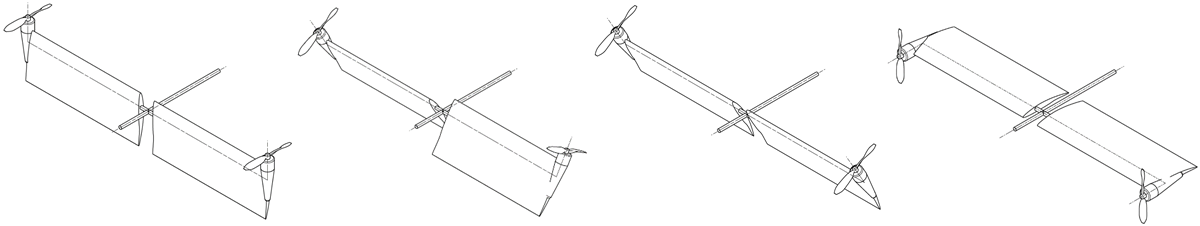
\includegraphics[width = \textwidth]{Tiltwing/TiltWingConfigurations.png}
    \caption[Range of tilt wing configurations]{Range of tilt wing configurations - from left: VTOL hover, VTOL yaw, VTOL Transition, Forward Flight}
    \label{fig:configs}
\end{figure}

\paragraph{VTOL System Requirements}
In the stationary hovering state, the angle of the wings relative to the body \(\theta_w\) will be approximately \(90\degree\) (zero along the $x$-axis). For control in the VTOL configuration, the tilt mechanism must be capable of inducing a positive and negative yawing moment on the UAV. To achieve this, the wings, and therefore the thrust of the wing-mounted motors, will need to be individually actuated and have a range of rotation beyond 90\degree. The maximum achievable angle will depend on the control scheme but is unlikely to exceed 135\degree (\citeauthor{inproceedings}, \citeyear{inproceedings}). \\

\paragraph{VTOL Transition System Requirements}
To achieve a controlled transition between the two flight modes, the transition phase will need to be rapid. Both wings will be required to tilt from an angle of approximately \(\theta_w=90\degree\) to approximately \(\theta_w=0\degree\) in unison and at the same rate. A separate single tilt mechanism, with rapid actuation, may be required for this.\\

\paragraph{Forward Flight System Requirements}
To allow the tilt-wing mechanism to be utilised for control during horizontal flight, a high degree of structural integrity and rotational angle accuracy is required. A design with a reliable and stable mechanism, with minimal moving parts is therefore desired. To allow control in forward flight and to eliminate the need of additional control surfaces, both wings will be required to have a tilt angle of approximately \(\theta_w=\pm5\degree\). Furthermore, due to increased cruise velocities and generally larger forces acting on the UAV during horizontal flight to VTOL transition, the tilt mechanism must be capable of withstanding large drag induced torques. Flight forces exceeding the maximum design torque of the tilt-wing will likely result in catastrophic failure. 

\subsubsection{Methodology}
A simplified analytical approach is taken to determine the external forces and resultant moments acing on the isolated tilt-wing mechanism. Understanding the potential moments around the $y$-axis will inform the design of the mechanism by indicating the required structural integrity and informing the operational requirements of potential actuating systems such as motors or servos. Moments around the $x$-axis and the $z$-axis are not as critical to the design of the tilt mechanism as the radial and axial loads they produce can be isolated through sturdy fuselage design and effective spar support through the use of bearings.

\subsubsection{Analysis}
A reference coordinate system relative to the body of the aircraft was generated to indicate the direction of acting forces. The origin of this coordinate system is indicated as $O$, and represents the center of the main spar, not the center of mass. Additionally, it is assumed that each wing has an individual central main spar running spanwise perpendicular to the fuselage. \\

\textbf{Forward Flight Configuration Modeling}
Figure \ref{fig:FFFBD} shows a static free body diagram of a tilt-wing during forward flight configuration. The averaged lift and drag forces of each aerofoil are functions of the linear velocities of the aircraft in the $x$ and $z$ directions, and the wing angle of attack. It is assumed that these forces act on the main spar ($y$-axis) of each wing and hence do not induce a moment around the $y$-axis at the origin. The forces produced by the port and starboard motors are assumed to act in the $x$ direction but along the $y$-axis and therefore do not produce a moment around the $y$-axis. The mass of the motors will cause a moment around the $y$-axis, but this will likely be small compared moments cause by external disturbances such as winds and gusts.\\
\begin{figure}[H]
    \centering
    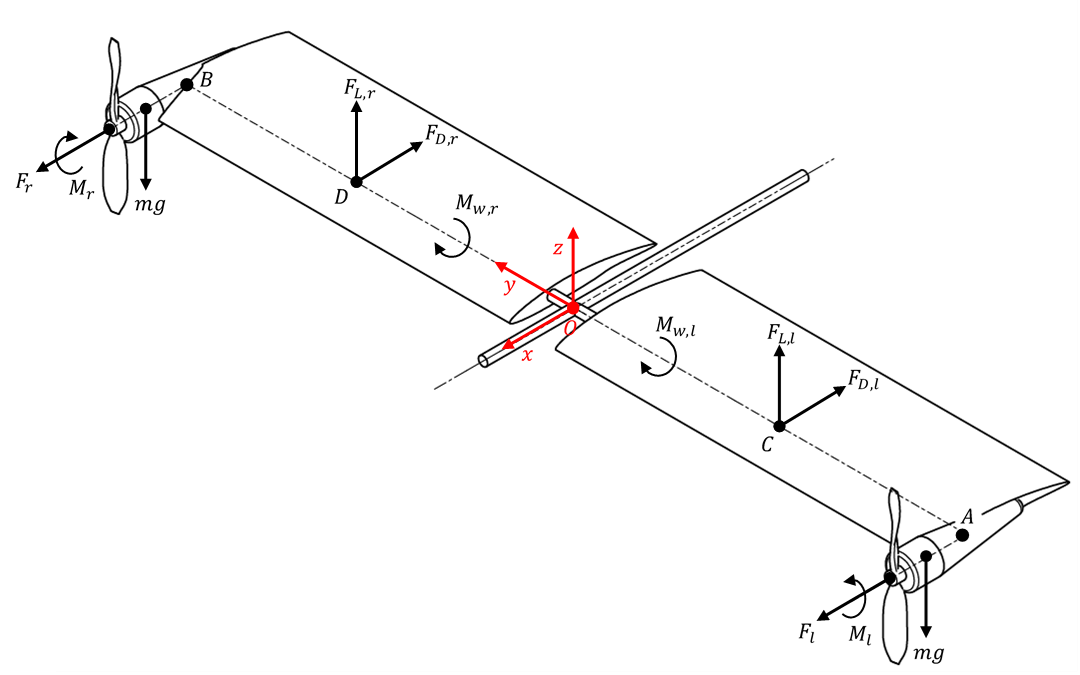
\includegraphics[width = \textwidth]{Tiltwing/FFFBD.png}
    \caption[Static Forward Flight FBD]{Static Forward Flight FBD of external forces and moments acting on an isolated tilt-wing system}
    \label{fig:FFFBD}
\end{figure}

\textbf{VTOL Configuration Modeling}
The static free body diagram of the VTOL configuration is depicted in Figure \ref{fig:VTOLFBD}. It displays similar forces as the forward flight configuration but in different orientations with respect to the coordinate system. The averaged lift and drag forces of each aerofoil are dependent on the vertical velocity in the $z$ direction. When hovering with a constant altitude these force are zero, but will develop with increasing vertical velocity. Similarly to the forward flight configuration, these forces are assumed to act along the main spars of each wing and hence do not induce a moment around the $y$-axis.\\
\begin{figure}[H]
    \centering
    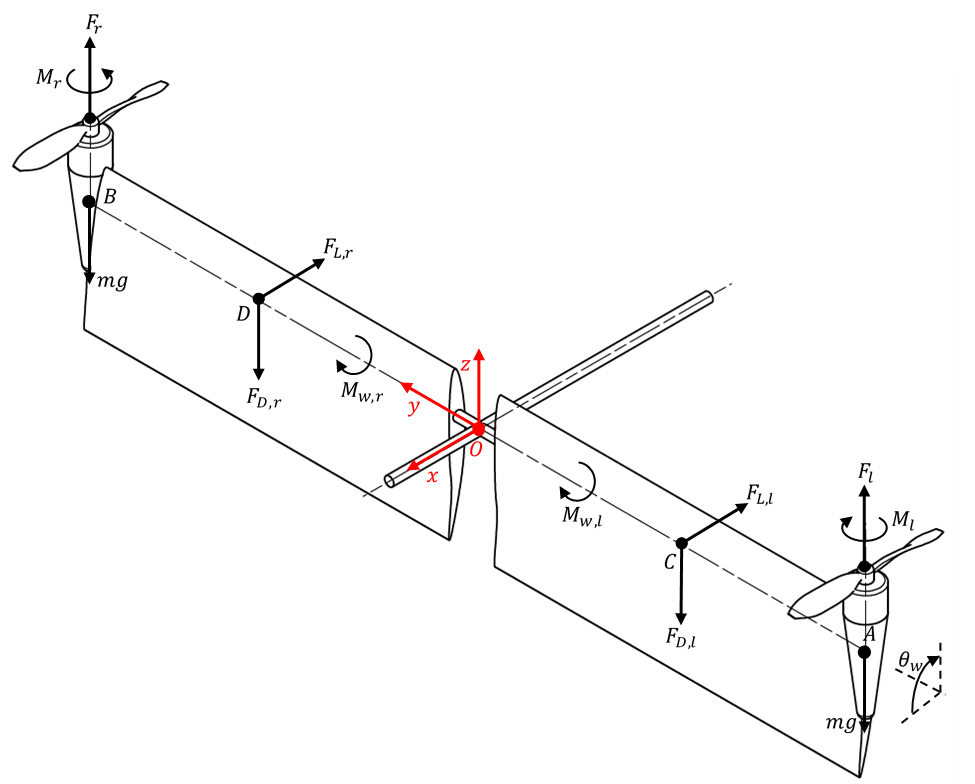
\includegraphics[width = \textwidth]{Tiltwing/VTOLFBD.png}
    \caption[Static VTOL FBD]{Static VTOL FBD showing the external forces and moments acting on an isolated tilt-wing system}
    \label{fig:VTOLFBD}
\end{figure}

\textbf{Worst Case Scenario Modeling}
The various forces and resultant moments of the two static configurations indicate minor torsional loads on the tilt-wing mechanism. During dynamic flight and VTOL transition however, the tilt mechanism will experience a larger spectrum of moments with greater amplitude. These will be created by shifting aerodynamic forces produced by the wings, external disturbances such as wind gusts and wing drag induced by VTOL transitioning. To simplify the modeling of such forces, a worst case scenario is considered. The torsional load of this scenario will occur when the aircraft suddenly transitions from forward flight to VTOL. In this scenario the two wings will quickly rotate from an angle of \(\theta_w=0\degree\) to \(\theta_w=90\degree\) relative to the body. The aerodynamic drag on the wings due to such a maneuver will induce large moments on the tilt mechanism.\\

By assuming the wings can be modeled as as a flat plate, the drag force can be calculated using Equation \ref{eqn:drag}.
\begin{equation}
    D=\frac{1}{2}C_D\rho v^2S \label{eqn:drag}
\end{equation}
% Where;
% \begin{eqnarray*}
%     C_D &=& \textnormal{coefficient of drag}\\
%     \rho &=& \textnormal{air density}\:[kg/m^3]\\
%     v &=& \textnormal{velocity of UAV}\:[m/s]\\
%     S &=& \textnormal{approximate surface area of the underside of the wing} \:[m^2]
% \end{eqnarray*}

The coefficient of drag is a function of several parameters including the shape of the body, Reynolds number of the flow, Froude number, Mach number and roughness of the surface. For simplification however the coefficient of drag of a flat plate perpendicular to the fluid flow was found from literature to equal 1.28. Assuming the VTOL transition occurs close to the ground, the density of air is assumed to equal 1.225 \(kg/m^3\). The surface area of the underside of the wing is calculated from analysis based on the wing loading and take off weight, resulting in a wing area (for both wings) approximately equal to \(0.54 m^2\). Assuming there is a control scheme to prevent VTOL transition at high cruise speeds, it is assumed that VTOL transition occurs at or near the stall speed of 12.5 m/s. The drag force for a single port or starboard wing can then be calculated as;
\begin{gather*}
    \therefore\quad D=1.28\times \frac{1}{2}\times 1.225\times 12.5^2\times \frac{0.54}{2} = 33.1 N
\end{gather*}
This drag force can be represented as a point force acting on the center of the wing underside. The location of this force relative to the location of the main spar determines the moment acting on the tilt mechanism. Current analysis has determined a MAC of approximately 0.3m. Therefore, assuming the main spar is located at a distance 25\% along the cord from the leading edge, the distance between the spar and the point drag force is 0.075m. This results in a moment of 2.51Nm acting on the tilt wing mechanism for a single port or starboard wing during a sudden VTOL transition. 

\subsubsection{Results} 
\paragraph{Design Requirements}
%talk about the torques ect determined from the modeling 
%talk about how different designs will require different servo torques
The worst case scenario analysis identified that the tilt wing mechanism must be capable of withstanding a torque of 2.51Nm. Furthermore, the system requirements identified that tilt angles ranging between \(-5\degree<\theta_w<135\degree\) are required for full control in both VTOL and forward flight. Therefore the total angular rotation of an actuating system must be capable of at least \(140\degree\) rotation.  \\
\\
\paragraph{Actuating Selection}
An array of actuators were considered to drive the tilt wings mechanism. These included common electric motor types such as; brushed and brush-less DC motors, stepper motors and positional rotation servo motors. The system requirements and design requirements were used determine the most suitable actuator for the tilt wing mechanism.\\
\\
Brushed/brush-less DC motors provide fast continuous rotation, ideal for use in worm drive or rack and pinion systems. When coupled with a rotary encoder, a highly accurate actuation system is possible. However, the tilt wing's dependence on positional awareness with high angular accuracy, supports the use of stepper motors and DC positional rotation servo motors. The use of such actuators is also suited towards this system as the required angle of rotation is only \(140\degree\leqslant\theta_w\leqslant180\degree\). Although stepper motors can accurately rotate with a high pole count ranging from 50 to 100, they too are intended for large angular rotation. Furthermore they have the potential to skip a pole, resulting in skewed accuracy. Their current consumption is also independent of load and hence constantly draw maximum current. DC positional rotation servos allow upwards of \(90\degree\) rotation in either direction for a total of \(180\degree\) or more movement, aligning well with the system requirements. A potentiometer coupled with a control circuit uses pulse width modulation (PWM) signals to control the position of the servo. This feedback system allows the servo to constantly correct any drift from the intended location. Servos are also generally able to generate higher peak torques than the holding torque of a stepper motor and are often smaller and more current efficient. In conclusion DC positional rotation servos present various advantages over other actuation mechanisms and although additional testing and analysis is required, were selected to actuate the prototype tilt wing mechanism. \\
\\
A large range of servos with varying torque ratings, construction materials and angular speeds are commercially available. Various servos exceed the required torque of 2.51 Nm \((25.6\text{ kg$\cdot$ cm})\) and a selection are displayed in Table \ref{tab:servos}. The range of potential servos suitable for the mechanism could also be increased through designs that harness mechanical advantage through leverage or gearing. A safety factor must also be considered.\\

\begin{table}[H]
\caption{Potential Servos for Tilt Wing Mechanism}
\label{tab:servos}
\centering
\resizebox{\textwidth}{!}{
\begin{tabular}{|l|l|l|l|l|l|}
\hline
\textbf{Part Number }& \textbf{Torque (kg-cm)} & \textbf{Speed (sec/60$^\circ$)} & \textbf{Weight (g)} & \textbf{Gears} \\ \hline
    SBRS-5314HTG & 53.1 & 0.18 sec/60$^\circ$ @ 7.4 V & 81 & Metal \\ \hline
    SPMSA6030 & 20 & 0.15 sec/60$^\circ$ @ 6.0 V & 52.4 & Titanium \\ \hline
    DS3225 & 25 & 0.13 sec/60$^\circ$ @ 6.8 V & 67 & Metal \\ \hline
\end{tabular}
}
\end{table}
\\
\paragraph{Preliminary Tilt Mechanism Design}
Based on the preliminary decision to utilise servos, a preliminary prototype tilt wing mechanism was designed. This prototype is a scaled version, designed to accommodate a Turnigy R5180MG analog servo. Due to the small servo size, the prototype was 3D printed for inspection and scaled operation testing. The mechanism allows for individual actuation of both wing spars, with a maximum servo rotation of \(180\degree\), easily meeting the angular rotation requirement of \(\theta_w\). Furthermore the system isolates the radial and axial loads of the wings through the use of bearings and allows for a modular wing design in which the wings can easily be detached from the system. Lastly, the mechanism can easily be modified to actuate a single spar spanning two wings which do not require individual actuation. An isometric view of the mechanism is displayed in Figure \ref{fig:render} and additional CAD drawings can be found in Appendix \ref{app_CAD}.
\begin{figure}[H]
    \centering
    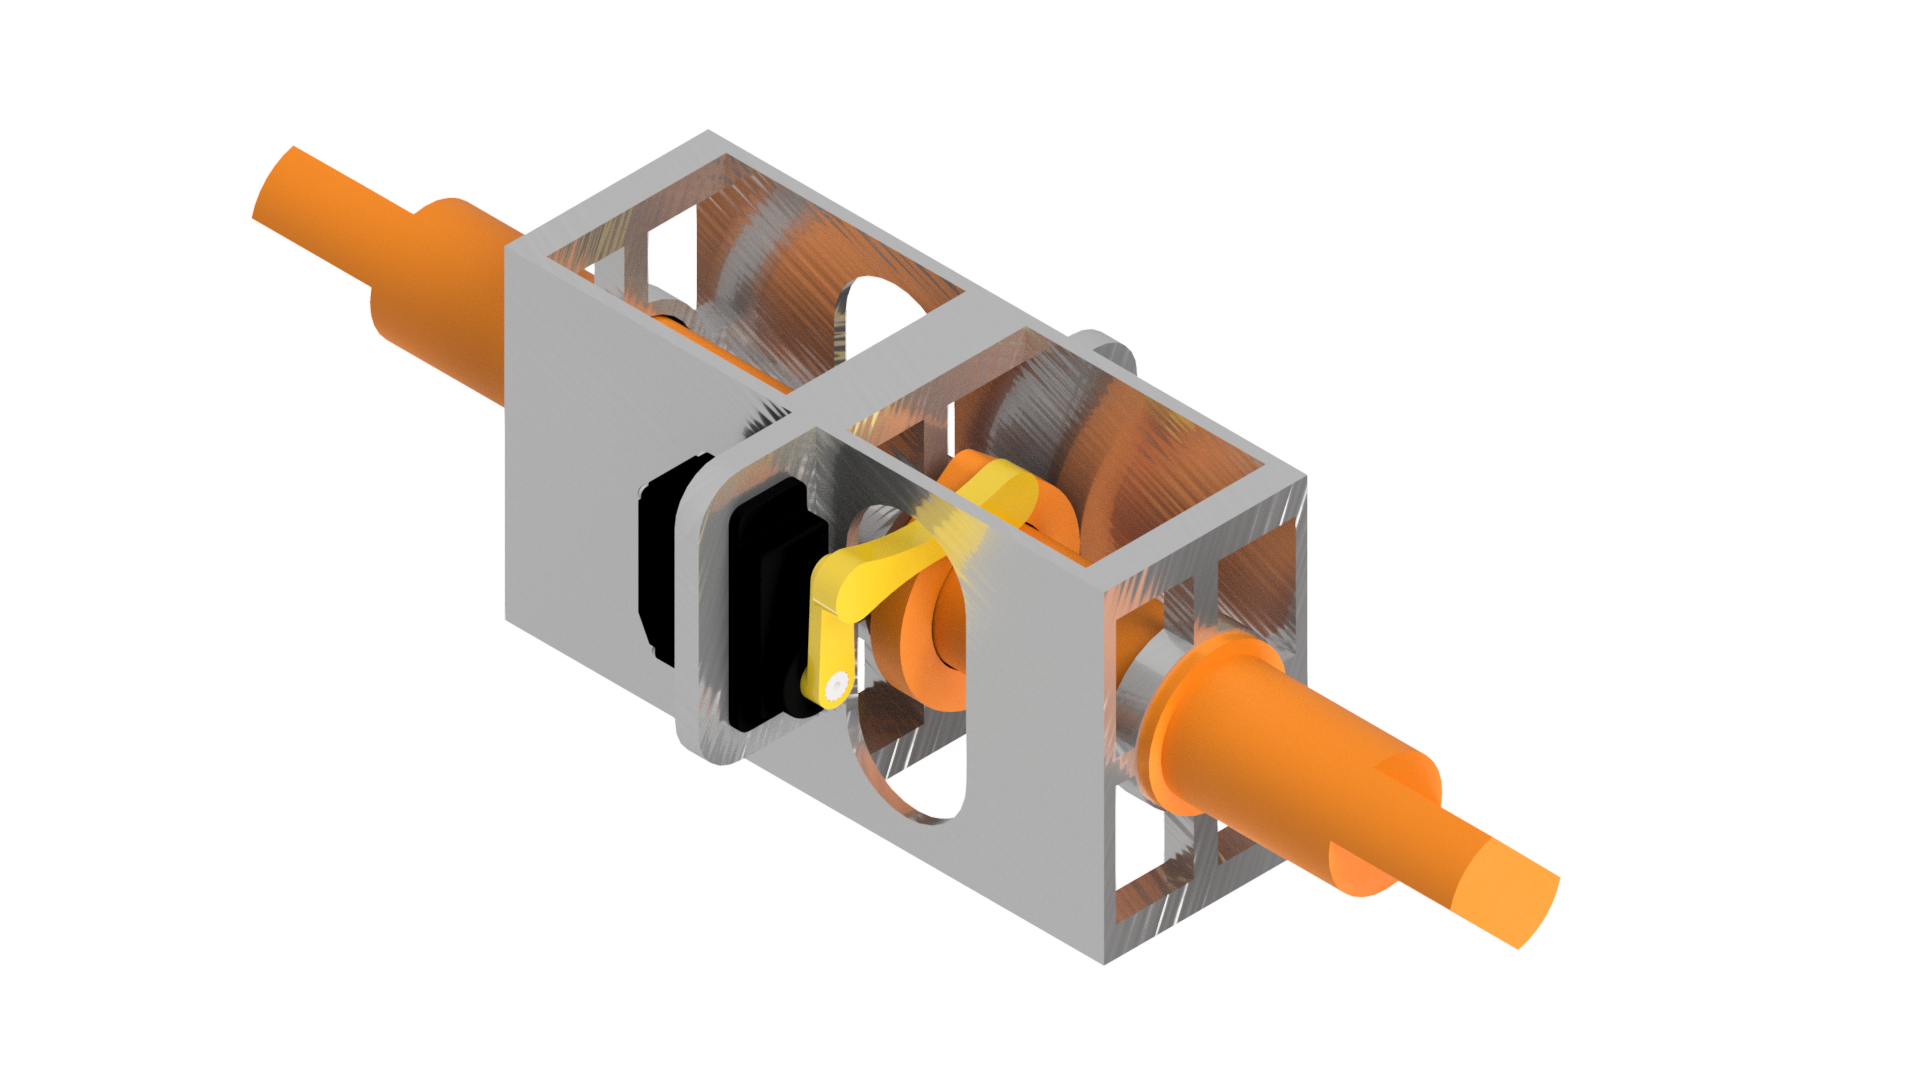
\includegraphics[width = \textwidth]{Tiltwing/Tilt Assembly Render.png}
    \caption{Rendered CAD of Prototype tilt-wing Mechanism}
    \label{fig:render}
\end{figure}

\subsubsection{Summary}
The tilt wing mechanism is a critical component of the VTOL UAV and hence requires in depth analysis to support design decisions prior to manufacturing. The subsystem is essential to the operational success of the UAV and failure to meet the subsystem requirements is likely to result in catastrophic failure. A basic analytical approach of a worst case scenario has been undertaken to calculate preliminary torques that a tilt wing mechanism must be capable of withstanding. A preliminary actuator type has also been selected and incorporated into a prototype tilt wing mechanism that can meet this torque requirement. 

\subsubsection{Future Work}
Additional testing of the prototype tilt wing mechanism is required to ensure intended functionality, full range of motion and other considerations such as voltage ranges and weight. The use of servos and the current prototype design is not final and could be subject to significant changes based on future analysis. Given the current prototype design is pursued and that it is subject to necessary modifications, designs can then begin for a full scaled prototype. This new prototype will be scaled up to house the selected servos, bearings and actual wing spars. Further discussion with the workshop will also be required to discuss manufacturing difficulties and tolerances. Once the full scale prototype is complete, an iterative testing and modification stage can commence. Torque testing using a torque wrench or spring force meter will be used in this phase to test the rated holding torque of the servos and system as a whole. Once the tilt-wing mechanism is operational and near optimal, further analysis using Datcom and potentially a wind tunnel can be used to experiment with wing angles of attack to optimise the efficiency and control of the system in all flight configurations. 
